
%(BEGIN_QUESTION)
% Copyright 2012, Tony R. Kuphaldt, released under the Creative Commons Attribution License (v 1.0)
% This means you may do almost anything with this work of mine, so long as you give me proper credit

If the free end of the rope is pulled a distance of 10 cm, how far will the mass be lifted?

$$\includegraphics[width=15.5cm]{i02629x01.eps}$$

Assuming the mass is 55 kg, how much work is done while pulling the rope 10 cm?

\underbar{file i02629}
%(END_QUESTION)





%(BEGIN_ANSWER)

Seeing that the lower pulley assembly is supported by {\it four} lengths of rope, the mechanical advantage in this system must be 4:1.  Thus, the output displacement will be four times less than the input displacement:

$$M_A = {x_{in} \over x_{out}}$$

$$x_{out} = {x_{in} \over M_A}$$

$$x_{out} = {10 \hbox{ cm} \over 4} = 2.5 \hbox{ cm}$$

Expressing the same result in meters instead of centimeters:

$$x_{out} = {0.1 \hbox{ m} \over 4} = 0.025 \hbox{ m}$$

\vskip 10pt

A mass of 55 kg weighs 539.99 newtons in Earth's gravity ($F = ma$, where $F$ is the force that gravity exerts on the mass, $m$ is the amount of mass, and $a$ is the acceleration of Earth gravity: 9.81 meters per second squared).  This is the amount of force exerted upward on the mass by the pulley system.  Given our mechanical advantage of 4:1, it means the rope's tension at the pulled end must be $1 \over 4$ this value, or 134.89 newtons.

\vskip 10pt

We may calculate the amount of work done at the mass or at the rope's end.  Either way, we will get the exact same result:

\vskip 10pt

$$W = F x = (134.89 \hbox{ N}) (0.1 \hbox{ m}) = 13.489 \hbox{ N-m \hskip 20pt (calculated at rope's end)}$$

$$W = F x = (539.55 \hbox{ N}) (0.025 \hbox{ m}) = 13.489 \hbox{ N-m \hskip 20pt (calculated at mass)}$$


%(END_ANSWER)





%(BEGIN_NOTES)


%INDEX% Machine, pulley
%INDEX% Machine, mechanical advantage
%INDEX% Physics, energy, work, power: calculating work and power

%(END_NOTES)


